\subsubsection*{Resultados del perceptron multicapa}

Como podíamos esperar, se produce un gran sobreajuste en el modelo por lo que no emplearemos ninguna de las métricas típicas para evaluarlo.

En su lugar mostraremos una gráfica que compare los labels de los audios con las predicciones del modelo.

\begin{figure}[htbp]
	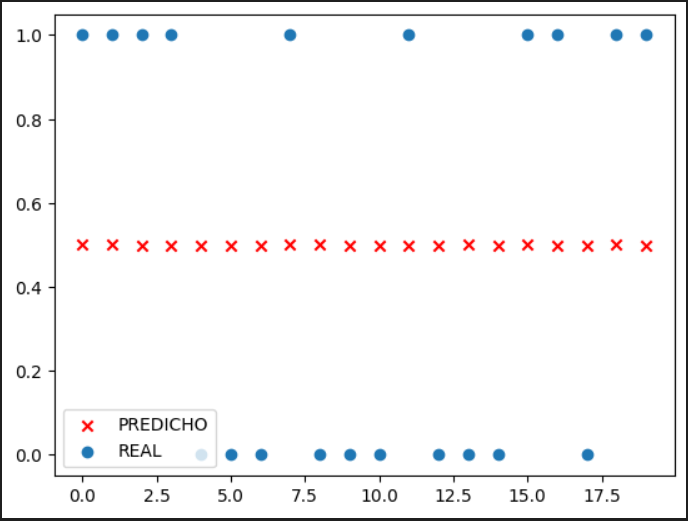
\includegraphics[width=\textwidth]{imagenes/Resultados_MLP.png}
	\caption{Resultados del MLP.}
	\label{fig:MLP}
\end{figure}

Las conclusiones que podemos sacar sobre este modelo a la vista de los resultados son que para crear un modelo de clasificación desde 0 y que sea eficaz en su labor, necesitaríamos muchísimos más audios de los que disponemos, además, en lo que se refiere a la posterior tarea de aplicar elementos de IA explicable al modelo, al usar embeddings como entrada, no podemos aplicarle directamente ninguna de esas técnicas.

Lamentablemente debido a estos resultados tomamos la decisión de que no merecía la pena perder tiempo aplicándole técnicas de ia explicable.
